\section{Systems of Differential Equations}
\begin{itemize}
    \item We can write systems of differential equations in terms of matrices. For example:
          \begin{equation}
              \bm{x}' = \begin{bmatrix}
                  -\frac{1}{2} & \frac{1}{4}  \\
                  \frac{1}{2}  & -\frac{3}{4}
              \end{bmatrix}\bm{x} + \begin{bmatrix}
                  300 \\ 300
              \end{bmatrix}
          \end{equation}
    \item We can have a new definition of equilibrium
          \begin{definition}
              An equilibrium of a system $\bm{x}'=A\bm{x}+\bm{b}$ is the values $\bm{x}=\begin{bmatrix}
                      x_1 \\ x_2
                  \end{bmatrix}$ such that
              \begin{equation}
                  0=\bm{x}'=A\bm{x}+\bm{b}
              \end{equation}
          \end{definition}
          \textit{Note:} These are also known as \textbf{critical points} sometimes.
    \item This is just a linear algebra problem, so the solution is just
          \begin{equation}
              \bm{x} = -A^{-1}\bm{b},
          \end{equation}
          but this only works if $A$ is invertible.
    \item \textbf{Direction Fields and Orbits:} Without solving an autonomous system, we can draw its \textbf{direction field}
          \begin{equation}
              \vec{F}(x) = A\vec{x}+b
          \end{equation}
          on a grid of points. By convention, we draw all vectors at the same length:
          \begin{itemize}
              \item
          \end{itemize}
          \begin{example}
              Suppose we have the differential equation
              \begin{equation}
                  \bm{x}'= \begin{bmatrix}
                      2 & -2 \\ -1&3
                  \end{bmatrix}\bm{x} + \begin{bmatrix}
                      300 \\ 300
                  \end{bmatrix}.
              \end{equation}
              We can find the direction vector at a point $\vec{x}=\begin{bmatrix}
                      200 \\ 900
                  \end{bmatrix}$ by plugging it in to get
              \begin{equation}
                  \begin{bmatrix}
                      x_1' \\ x_2'
                  \end{bmatrix} = \bm{x}' = \begin{bmatrix}
                      2 & - 2 \\ -1 & 3
                  \end{bmatrix}\begin{bmatrix}
                      200 \\ 900
                  \end{bmatrix} + \begin{bmatrix}
                      300 \\ 300
                  \end{bmatrix} = \begin{bmatrix}
                      -1100 \\ 2800
                  \end{bmatrix},
              \end{equation}
              which after normalizing gives
              \begin{equation}
                  \begin{bmatrix}
                      -0.37 \\ 0.93
                  \end{bmatrix}
              \end{equation}
              For example, the phase portrait looks like
              \begin{center}
                  \def\length{sqrt((2*x-2*y+300)^2+(-1*x+3*y+300)^2)}

                  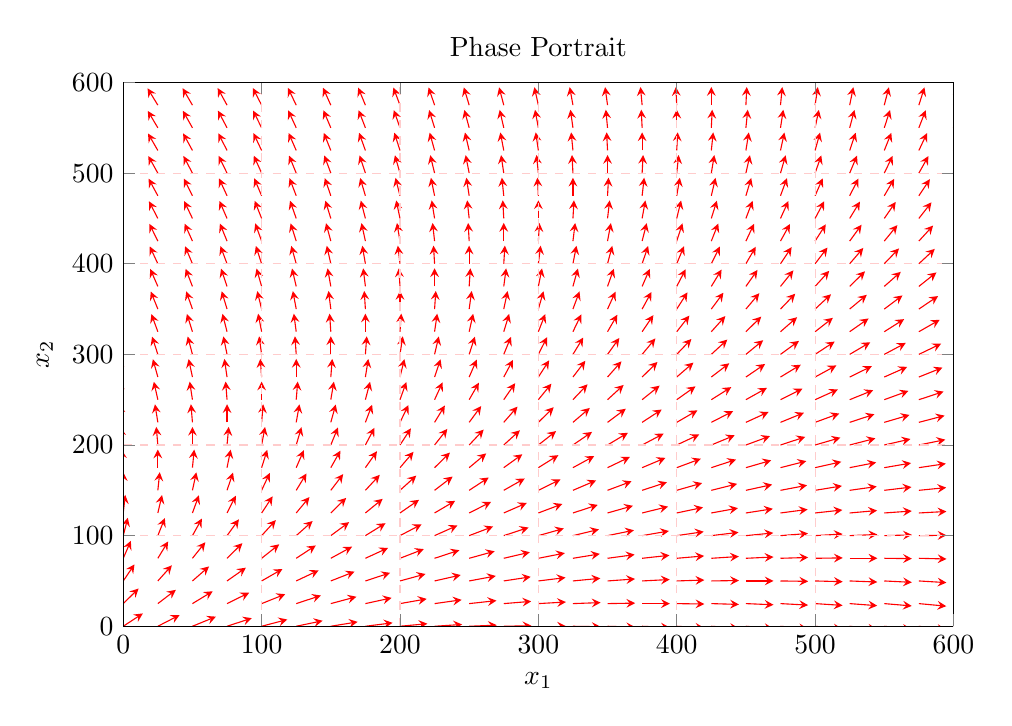
\begin{tikzpicture}

                      \begin{axis}[
                              grid=both,
                              grid style={dashed,red!20},
                              xmin = 0, xmax = 600,
                              ymin = 0, ymax = 600,
                              width = \textwidth,
                              height = 0.7\textwidth,
                              xlabel = {$x_1$},
                              ylabel = {$x_2$},
                              title={Phase Portrait},
                              view = {0}{90},
                          ]

                          % Vector Field
                          \addplot3[
                              quiver = {
                                      u = {(2*x-2*y+300)/\length},
                                      v = {(-1*x+3*y+300)/\length},
                                      scale arrows = 20,
                                  },
                              -stealth,
                              domain = 0:600,
                              domain y = 0:600,
                              red
                          ]
                          {0};

                      \end{axis}
                  \end{tikzpicture}
              \end{center}
              From this, we can see how initial conditions can determine the end conditions.
          \end{example}
    \item A \textbf{homogenous system} is when $\bm{b}=0.$
    \item We can reduce a non-homogenous system to a homogenous system. Let us write
          \begin{equation}
              \bm{x}=\bm{\phi} + \bm{q}.
          \end{equation}
          where $\bm{q}$ is the equilibrium. Then\footnote{This is similar to how in PHY293, we were able to modify the differential equation for a spring-mass system with gravity, and remove the gravity component by changing coordinates.}:
          \begin{align}
              \bm{x}' = A\bm{x}+\bm{b} & \iff \bm{\phi}' = A(\bm{\phi}+\bm{q})+\bm{b}                                                  \\
                                       & \iff \bm{\phi}' = A\bm{\phi} + \underbrace{A\bm{q} + A\bm{b}}_{\text{zero since equilibrium}} \\
                                       & \iff \bm{\phi}' = A\bm{\phi}
          \end{align}
          \begin{idea}
              Every solution of the non-homogenous problem can be written as a solution of the homogenous problem plus the equilibrium.
          \end{idea}
          \begin{example}
              Consider the system $\bm{x}' = \begin{bmatrix}
                      4 & -2 \\ 3 & -3
                  \end{bmatrix}\bm{x}.$ Then we can verify that
              \begin{equation}
                  \bm{x} = \begin{bmatrix}
                      1 \\ 3
                  \end{bmatrix}e^{-2t}
              \end{equation}
              solves this system by directly substitution. We can also verify that
              \begin{equation}
                  \bm{x} = \begin{bmatrix}
                      2 \\ 1
                  \end{bmatrix}e^{3t}
              \end{equation}
              solves this equation as well. However, what is more interesting is that any linear combination of these two solutions is also a solution: and thus it is more general.
          \end{example}
          \begin{theorem}
              \textbf{Superposition Principle:} Suppose $\bm{\phi_1}$ and $\bm{\phi_2}$ are solutions to $\bm{x}'=A\bm{x}$. Then for any coefficients $c_1$ and $c_2$, this is also a solution:
              \begin{equation}
                  \bm{\phi}(t) = c_1\bm{\phi_1}(t) + c_2\bm{\phi_2}(t)
              \end{equation}
              Alternatively, the set of solutions to $\bm{x}'=A\bm{x}$ is a subspace of functions.
          \end{theorem}
    \item It turns out that the subspace of solutions to $\bm{x}'=A\bm{X}$ is always two-dimensional if it is a system of two equations.
          \begin{definition}
              Two functions $\bm{\phi_1}$ and $\bm{\phi_2}$ are linearly independent if and only if
              \begin{equation}
                  c_1\bm{\phi_1}+c_2\bm{\phi_2} = 0 \implies c_1=c_2 = 0.
              \end{equation}
          \end{definition}
          \begin{example}
              We can show that $\bm{\phi_1}=\begin{bmatrix}
                      e^t \\ e^{-t}
                  \end{bmatrix}$ and $\bm{\phi_2} = \begin{bmatrix}
                      \sin t \\ e^{-t}
                  \end{bmatrix}$ are linearly independent because
              \begin{equation}
                  c_1\bm{\phi_1}+c_2\bm{\phi_2} = 0 \implies \begin{cases}
                      c_1e^t + c_2\sin t = 0 \\
                      c_1e^{-t} + c_2e^{-t} = 0
                  \end{cases}
              \end{equation}
              This linear system gives
              $c_1=c_2=0.$
          \end{example}
          \begin{theorem}
              The solutions $\bm{\phi_1}(t) =\begin{bmatrix}
                      x_{11}(t) \\ x_{21}(t)
                  \end{bmatrix}$ and $\bm{\phi_2}(t) =\begin{bmatrix}
                      x_{12}(t) \\ x_{22}(t)
                  \end{bmatrix}$  of $\bm{x}'=A\bm{x}$ are linearly independent if and only if the Wronskian is nonzero:
              \begin{equation}
                  W[\bm{\phi_1},\bm{\phi_2}] = \det\begin{bmatrix}
                      x_{11}(t) & x_{12}(t) \\
                      x_{21}(t) & x_{22}(t)
                  \end{bmatrix} \neq 0
              \end{equation}
              for all $t\in I$.
          \end{theorem}
          \begin{example}
              Let's solve $\bm{\phi}'=A\bm{\phi}$ where $A=\begin{bmatrix}
                      -1/2 & 1/4 \\
                      1/2        \\ -3/4
                  \end{bmatrix}.$ We can use an educated guess: $\bm{\phi} = e^{\lambda t}\bm{v}$ for some vector $\bm{v}$. If we substitute this in, we get
              \begin{equation}
                  A\bm{\phi} = \lambda \bm{\phi}
              \end{equation}
              We can solve for the eigenvalue and eigenvectors to get 
              \begin{align}
                  \bm{\phi_1} &= e^{-(1/4) t} \begin{bmatrix}
                      1 \\ 1
                  \end{bmatrix} \\ 
                  \bm{\phi_2} &= e^{-t}\begin{bmatrix}
                      -1/2 \\ 1
                  \end{bmatrix}
              \end{align}
              Finally, we need to check the Wronskian is nonzero (it is). The general solution is thus: 
              \begin{equation}
                  x(t) = \begin{bmatrix}
                      1200 \\ 1200
                  \end{bmatrix} + c_1e^{-(1/4)t}\begin{bmatrix}
                      1\\ 1
                  \end{bmatrix} + c_2e^{-t}\begin{bmatrix}
                      -1/2 \\ 1
                  \end{bmatrix}
              \end{equation} 
          \end{example}
          \item We can look at some casework where we have two distinct eigenvalues: 
          \begin{itemize}
              \item $\lambda_1,\lambda_2 < 0$
              \begin{itemize}
                  \item Critical Point(s): $(0,0)$ only.
                  \item Stable equilibrium 
              \end{itemize}
              \item $\lambda_1,\lambda_2 > 0$
              \begin{itemize}
                  \item Critical Point(s): $(0,0)$ only.
                  \item Unstable Equilibrium
              \end{itemize}
              \item $\lambda_1 > 0 > \lambda_2$
              \begin{itemize}
                  \item 
              \end{itemize}
              \item $\lambda_1 = 0$, $\lambda_2 < 0$
              \begin{itemize}
                  \item Equilibrium: The line associated with $\lambda_1=0.$
              \end{itemize}
          \end{itemize}
          Note that the $\lambda_1 =0, \lambda_2>0$ case is not covered, but it is similar to the fourth case.
\end{itemize}